% TEMPLATE for Usenix papers, specifically to meet requirements of
%  USENIX '05
% originally a template for producing IEEE-format articles using LaTeX.
%   written by Matthew Ward, CS Department, Worcester Polytechnic Institute.
% adapted by David Beazley for his excellent SWIG paper in Proceedings,
%   Tcl 96
% turned into a smartass generic template by De Clarke, with thanks to
%   both the above pioneers
% use at your own risk.  Complaints to /dev/null.
% make it two column with no page numbering, default is 10 point

% Munged by Fred Douglis <douglis@research.att.com> 10/97 to separate
% the .sty file from the LaTeX source template, so that people can
% more easily include the .sty file into an existing document.  Also
% changed to more closely follow the style guidelines as represented
% by the Word sample file. 

% Note that since 2010, USENIX does not require endnotes. If you want
% foot of page notes, don't include the endnotes package in the 
% usepackage command, below.



% Good read: https://www.usenix.org/legacy/events/samples/template.la
\documentclass[letterpaper,twocolumn,10pt]{article}
\usepackage{usenix,epsfig,endnotes}
\begin{document}

%don't want date printed
\date{}

%make title bold and 14 pt font (Latex default is non-bold, 16 pt)
\title{ RL-Competition: Lambda sarsa agent\\ \small a submission to the competition in ``Decision making under uncertainty``}

\author{
{\rm John Karlsson}\\
kajohn@student.chalmers.se
\and
{\rm Oscar Carlsson}\\
coscar@student.chalmers.se
\and
{\rm Oskar Lindgren}\\
rockoskar@chalmers.se
}

\maketitle

% Use the following at camera-ready time to suppress page numbers.
% Comment it out when you first submit the paper for review.
\thispagestyle{empty}


\subsection*{Abstract}
Agent using: Sarsa lambda, KL-USB, Tiebraker \\
Experiments: Tictactoe MDP, Connectfour POMDP \\
Results..

\section{Introduction}
This report details our submission to the Reinforcement Learning competition held in the course ``Decision making under uncertainty``~\cite{RLCOMP}. The competition was to implement a agent that would communicate with rl glue~\cite{rl-glue} and act in environments with discrete state spaces.

%\endnote{Remember to use endnotes, not footnotes!} galore, plethora of promises.\\

\section{Environments}
In addition to the implemented agent we've implemented two environments representing the board games ticktacktoe and connect four. The ticktacktoe environment is a fully observable Markov Decision Process (MDP) whilst connect four is a Partially observable MDP (POMDP).
\paragraph{Tic-tac-toe}
Number of states: 19683 \\
Number of actions: 9\\
Reward space : -10 to 10.\\
\\
The states are represented by a integer calculated as..\\
\\
Agent fills the board: 1\\
Agent wins: 10\\
Illegal move: -10\\
AI wins: -1
\paragraph{Connect four}
Number of states: 2188 \\
Number of actions: 7\\
Reward space : -1 to 1\\
\\
The states are represented by a integer calculated as..\\
\\
Illegal move: -1\\
The board is full:  0\\
AI wins: 0\\
Agent wins: 1
\section{The Agent}
We use everything from~\cite{Sutton:1998:IRL:551283}
\paragraph{Sarsa lambda}
Lorem ipsum dolor sit amet, consectetur adipiscing elit, sed do eiusmod tempor incididunt ut labore et dolore magna aliqua. Ut enim ad minim veniam, quis nostrud exercitation ullamco laboris nisi ut aliquip ex ea commodo consequat. 
\paragraph{Tiebreaker}Indeed we did.Lorem ipsum dolor sit amet, consectetur adipiscing elit, sed do eiusmod tempor incididunt ut labore et dolore magna aliqua. Ut enim ad minim veniam, quis nostrud exercitation ullamco laboris nisi ut aliquip ex ea commodo consequat. 
\paragraph{KL-UCB}Wanna know more?~\cite{DBLP:journals/jmlr/GarivierC11}Lorem ipsum dolor sit amet, consectetur adipiscing elit, sed do eiusmod tempor incididunt ut labore et dolore magna aliqua. Ut enim ad minim veniam, quis nostrud exercitation ullamco laboris nisi ut aliquip ex ea commodo consequat. 
\section{Results}
All code is found at https://github.com/Oscarlsson/RL-competition

Choosing $\lambda$
\begin{figure}[h]
    \centering
    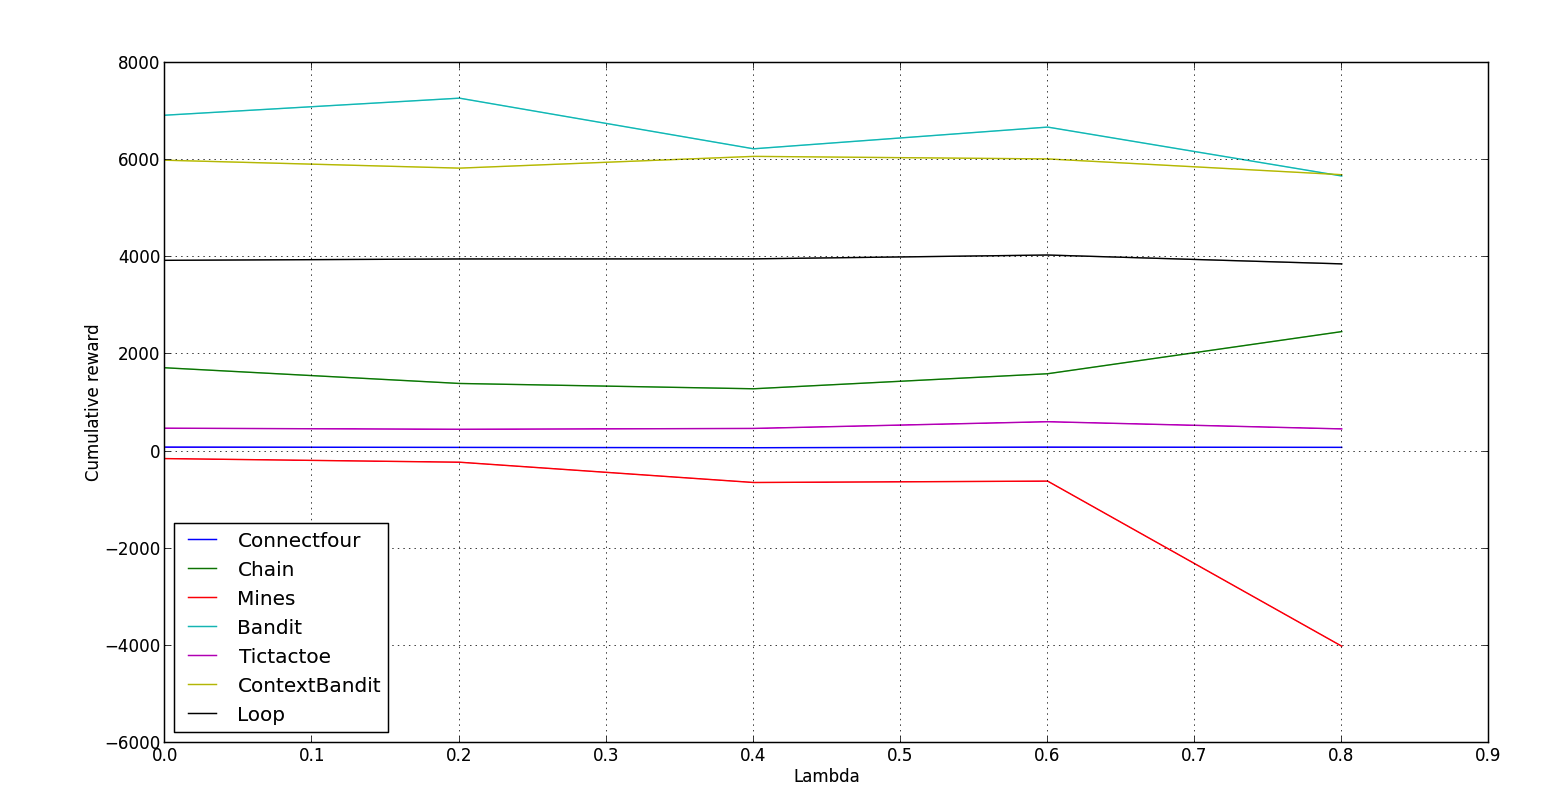
\includegraphics[width=0.5\textwidth]{../data/lambdasweepplotTEST.png}
    \caption{Awesome Image}
    \label{fig:awesome_image}
\end{figure}


Our agent in a 100 episode run against all environments with $\lambda = 0.2$ and $\alpha = 1$
\begin{figure}[h]
    \centering
    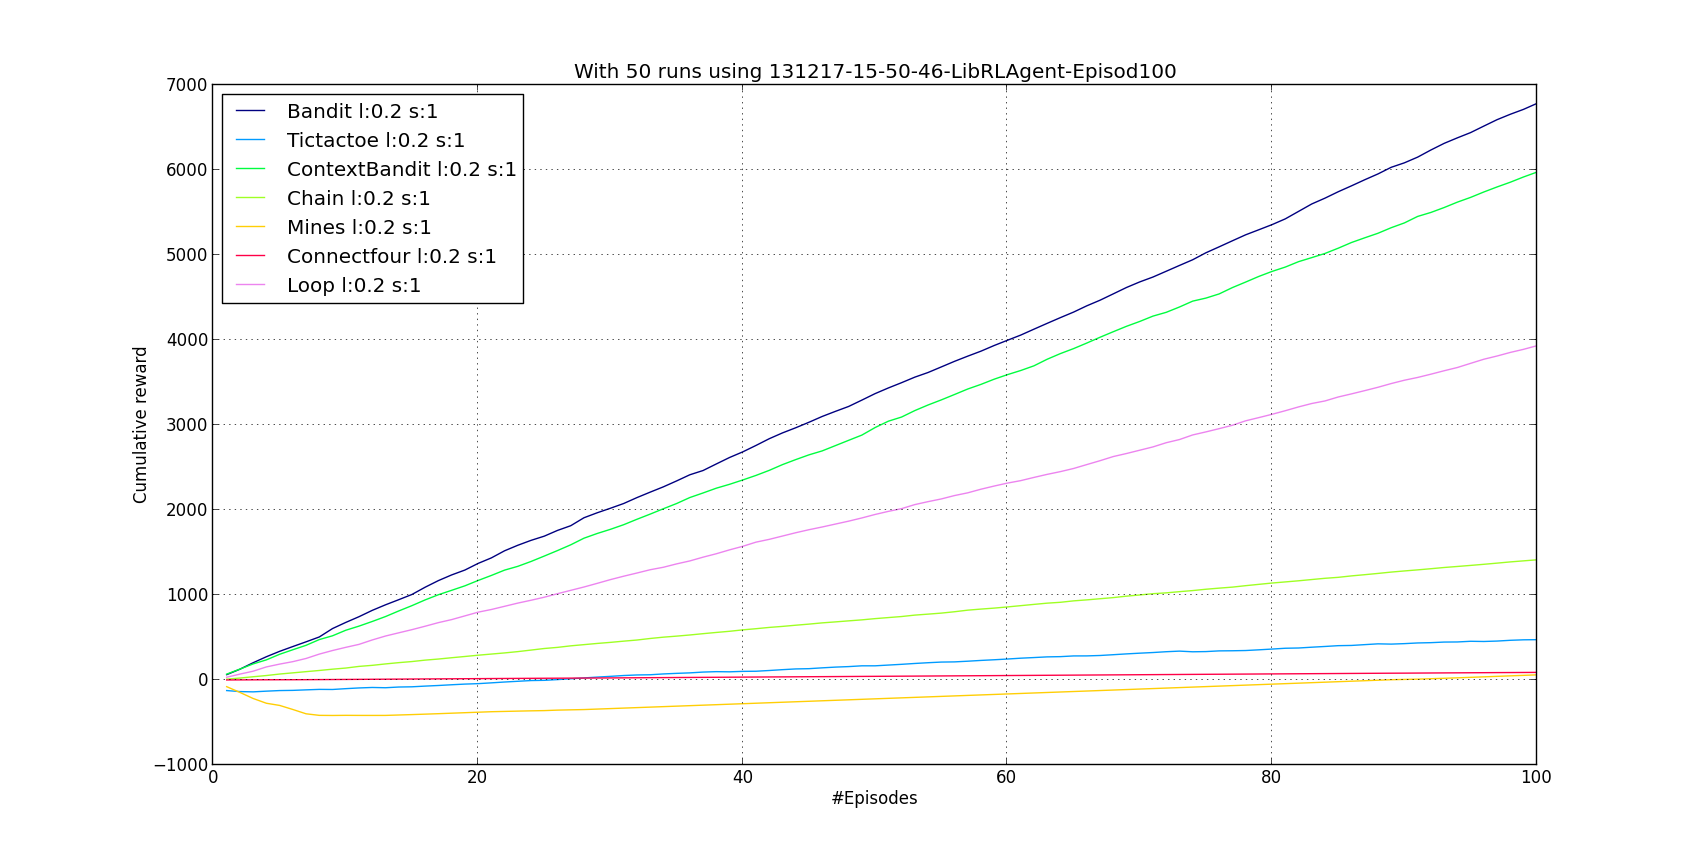
\includegraphics[width=0.5\textwidth]{../data/100episodes_50runs.png}
    \caption{Awesome Image}
    \label{fig:awesome_image}
\end{figure}

{\footnotesize \bibliographystyle{acm}
\bibliography{sample}}


\theendnotes

\end{document}







